\documentclass[10pt]{ijgtp}

\usepackage{cmap,amsmath,amssymb}
\usepackage[utf8]{inputenc}
\usepackage[T1]{fontenc}
\usepackage[english]{babel}
\usepackage{lipsum}

\begin{document}

%\arxivnumber{2026.0000}

\title{Title of the manuscript}

\author{First Lastname}
\affiliation{Affiliation 1}
\affiliation{Affiliation 2}
\email{email1@uni.edu}
%\orcid{0000-0000-0000-0000}

\author{Corresponding Person}
\affiliation{Affiliation 2}
\affiliation{Affiliation 3}
\email{email2@uni.edu}
%\orcid{0000-0000-0000-0000}
\corresponding

\begin{abstract}
This is an abstract.

\lipsum[1-2]
\end{abstract}

%\pacs{02.30.Mv; 04.30.-w; 04.50.Gh; 04.70.Bw}
\keywords{list of keyword}

\maketitle
\tableofcontents

\section{Introduction}
\label{sec:introduction}
This is the introduction. \lipsum[1-5]

\section{First section}
\label{sec:first}

\subsection{First subsection}
\label{sec:first-subsection}

\lipsum[1-2]

\subsection{Second subsection}
\label{sec:second-subsection}

\lipsum[1-3]

\section{Demonstrations}
\label{sec:demo}
This is an example of a citation \cite{Konoplya:2025uta,Matyjasek:2026yiu}.

Sections~\ref{sec:introduction} and~\ref{sec:first} provide the context for
this example; see also Subsection~\ref{sec:first-subsection}.
Equation~\eqref{eq:decay}, Table~\ref{tab:decay}, and Figure~\ref{fig:decay}
illustrate numbered objects and cross-references. The values below are
illustrative, rather than experimental results.

For a quantity with initial amplitude $A_0$ and decay time $\tau>0$, consider
\begin{equation}
  A(t)=A_0\exp\!\left(-\frac{t}{\tau}\right), \qquad t\geq 0.
  \label{eq:decay}
\end{equation}
Table~\ref{tab:decay} lists selected values of Equation~\eqref{eq:decay},
while Figure~\ref{fig:decay} shows the continuous curve.

\begin{table}%[htbp]
  \centering
  \begin{tabular}{cc}
    \hline
    $t/\tau$ & $A(t)/A_0$ \\
    \hline
    0 & 1.0000 \\
    1 & 0.3679 \\
    2 & 0.1353 \\
    3 & 0.0498 \\
    \hline
  \end{tabular}
  \caption{Illustrative normalized amplitudes for exponential decay.}
  \label{tab:decay}
\end{table}

\begin{figure}%[htbp]
  % LaTeX uses sample-figure.eps; PDFLaTeX uses the matching PDF.
  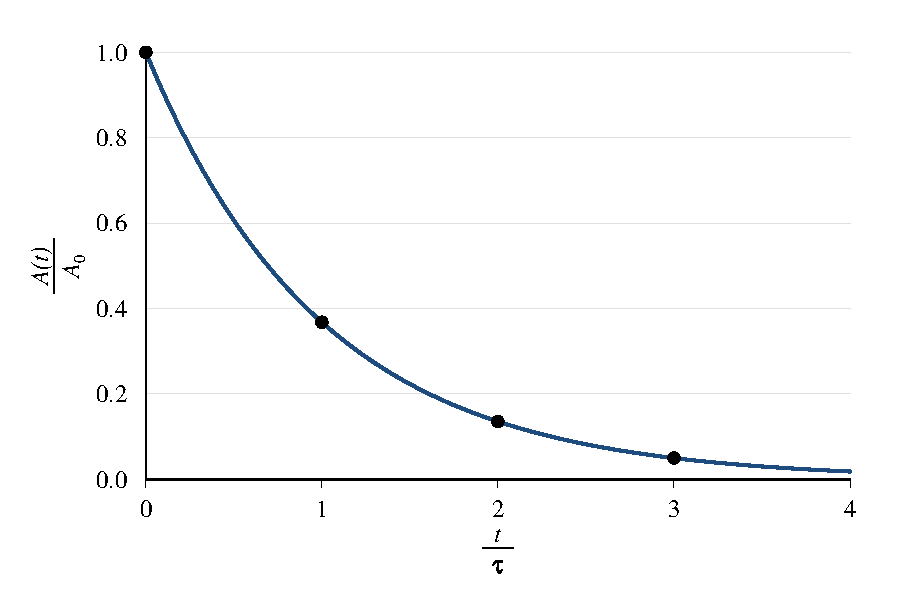
\includegraphics[width=\linewidth]{sample-figure}
  \caption{Exponential decay given by Equation~\eqref{eq:decay}.
    The markers correspond to the values in Table~\ref{tab:decay}.}
  \label{fig:decay}
\end{figure}

Section~\ref{sec:conclusions} concludes the manuscript.

\section{Conclusions}
\label{sec:conclusions}
Section~\ref{sec:demo} demonstrates the sample equation, table, and figure.
In conclusion, \lipsum[1]

\section*{Author Contributions}
F.L.: conceptualization, methodology, software, writing; C.P.: conceptualization, methodology, software, writing. All authors have read and agreed to the published version of the manuscript.

\section*{Funding}
This paper was supported by a Funding agency.

\section*{Institutional Review Board Statement}
Not applicable.

\section*{Informed Consent Statement}
Not applicable.

\section*{Data Availability Statement}
Not applicable.

\section*{Conflicts of Interest}
The authors declare no conflict of interests.

\section*{Use of AI and AI-Assisted Technologies}
During the preparation of this work, the authors used ChatGPT developed by OpenAI for language editing and text refinement. After using this service, the authors reviewed and edited the content as needed and take full responsibility for the content of the published article.

\bibliography{template}
\end{document}
